\section{Expériences numériques}

Pour simuler notre four à micro-ondes efficace il faut préciser le domaine
(dimensions du four) et les constantes qui apparaissent dans les équations de
Helmholtz et Poisson.

\subsection{Constantes}
\label{experiences_numeriques:constantes}

La perméabilité magnétique relative $\mu$ est très proche de
1.0 dans l'air et dans l'eau. Et comme le teneur de l'eau dans les aliments est
environ 70\% on peut supposer que
\begin{align}
    \mu = 1.0
\end{align}

La permittivité relative $\epsilon$ est égale à 1.0 dans l'air et 4.0 dans
l'eau, et donc 4.0 dans l'aliment. Toutefois, pour avoir une solution complexe
de l'équation de Helmholtz, on ajoute une partie imaginaire à la
permittivité relative. Après quelques expériences numériques avec des parties
complexes différentes, on a choisi les valeurs suivantes :
\[\begin{dcases}
    \epsilon(x) = 1 - 0.05i & x \text{ dans l'air} \\
    \epsilon(x) = 4(1 - 0.05i) & x \text{ dans l'objet à cuire}
\end{dcases}\]

La conductivité thermique $K$ est égale à 0.0262 dans l'air et 0.6 dans
l'eau, et donc 0.6 dans l'aliment :
\[\begin{dcases}
      K(x) = 0.0262 & x \text{ dans l'air} \\
      K(x) = 0.6 & x \text{ dans l'objet à cuire}
\end{dcases}\]

% =============================================================================

\subsection{Dimensions du four}
\label{experiences_numeriques:dimensions_four}

La taille de notre four est 40cm $\times$ 30cm $\times$ 30cm. Ce
sont des dimensions plus ou moins en lignes avec les dimensions
des fours à micro-ondes standards. On utilise l'unité du centimètre
car c'est une échelle convenable pour la génération des maillages
et les figures.

\subsection{Fréquence des ondes électromagnétiques}

Pour qu'on ait une distribution efficace du champ électromagnétique
dans l'enceinte du four, il faut calibrer la fréquence des ondes
électromagnétiques émises par le magnétron. Par ailleurs, puisque le
magnétron se trouve derrière un des côtés
latérales de l'enceinte, les ondes électromagnétiques se déplacent
horizontalement. Donc, l'intensité des ondes dépend seulement de la
longueur (40cm) de l'enceinte.

Les fours à micro-ondes standards se servent des magnétrons qui émettent
des ondes électromagnétiques à une fréquence de 2.45 GHz. Avec une telle
fréquence le nombre de longueurs d'onde dans l'enceinte
est environ 3.

Avec cette fréquence la vitesse angulaire est très élevée :
$\omega = 2 \pi \times 2.45 \times 10^9 = \pi \times 4.9 \times 10^9$.
On aura donc dans l'équation de Helmholtz la quantité $\omega^2 \approx 10^{20}$.
Malheureusement, une valeur aussi élevée complique les calculs
numériques. En particulier, on utilise la valeur $10^{30}$ pour imposer
des conditions aux limites (la méthode de pénalisation). Pour éviter ce
souci on va manipuler les unités. Comme les constantes $\mu$ et
$\epsilon$ sont sans unités il
suffit juste de jouer avec la vitesse de la lumière.
Comme les dimensions du four sont définies en centimètres, il est
convenable de poser que la vitesse de la lumière $c = 1\frac{\text{cm}}{\text{s}}$.
Cela implique que, dans notre système d'unités, 1 mètre vaut
$3 \times 10^{10}$ mètres du système métrique standard.

On est à present en mesure de calculer une bonne fréquence pour
notre four. Soit $L$ la longueur de l'enceinte et $n_\lambda$
le nombre désiré de longueurs d'ondes (en centimètres).
La longueur d'onde est donc $\lambda = L / n_\lambda$, et on en tire
la fréquence,
\begin{align}
    f = \frac{c}{\lambda} = \frac{1}{\lambda} = \frac{n_\lambda}{L}
\end{align}

%Comme on impose des conditions aux limites de Dirichlet homogène, la
%magnitude du champ du côté opposé du magnétron est zéro.

Avec $n_\lambda = 2$, par exemple, la vitesse angulaire est donc
\begin{align}
    \omega = 2 \pi f = \frac{2 \pi n_\lambda}{L}
    = \frac{4 \pi}{40} = \frac{\pi}{10} \approx 0.314
\end{align}

% =============================================================================

\subsection{Conditions aux limites}

Le magnétron se trouve derrière la paroi gauche de l'enceinte du four, et
on applique alors des conditions aux limites au plan $x = -20$. Il reste à
déterminer les conditions aux limites appliquées aux 5 autres parois. On a
effectivement 2 options : soit on a $g = 0$ sur les autres parois, soit on
ne précise pas la valeur de $g$ sur les autres parois.

On va effectuer des expériences numériques pour ces 2 cas, mais on remarque
que le deuxième cas est plus réaliste. En effet, dans un four à micro-ondes
les ondes électromagnétiques réfléchissent contre les parois et la magnitude
du champ électromagnétique varie beaucoup sur la paroi.

On choisit comme fonction $g$ une espèce de pyramide tronquée d'une
hauteur de 1. Pour le premier cas indiqué plus haut on a
\[\begin{dcases}
    g(x, \tilde{y}, \tilde{z})
    = \min(4\tilde{y}, 4(1-\tilde{y}), 4\tilde{z}, 4(1-\tilde{z}), 1)
    & \text{si } x = -20 \\
    g(x, \tilde{y}, \tilde{z}) = 0 & \text{si } x \neq -20
\end{dcases}\]
%
Et pour le deuxième cas :
\begin{align}
      g(x, \tilde{y}, \tilde{z})
      = \min(4\tilde{y}, 4(1-\tilde{y}), 4\tilde{z}, 4(1-\tilde{z}), 1)
      \qquad \text{si } x = -20
\end{align}

où $\tilde{y}$ et $\tilde{z}$ sont les coordonnées normalisées au carré
$[0,1] \times [0,1]$ :
\begin{align}
    \tilde{y} = \frac{y + 15}{30} \qquad \tilde{z} = \frac{z + 15}{30}
\end{align}

\begin{figure}[H]
    \centering
    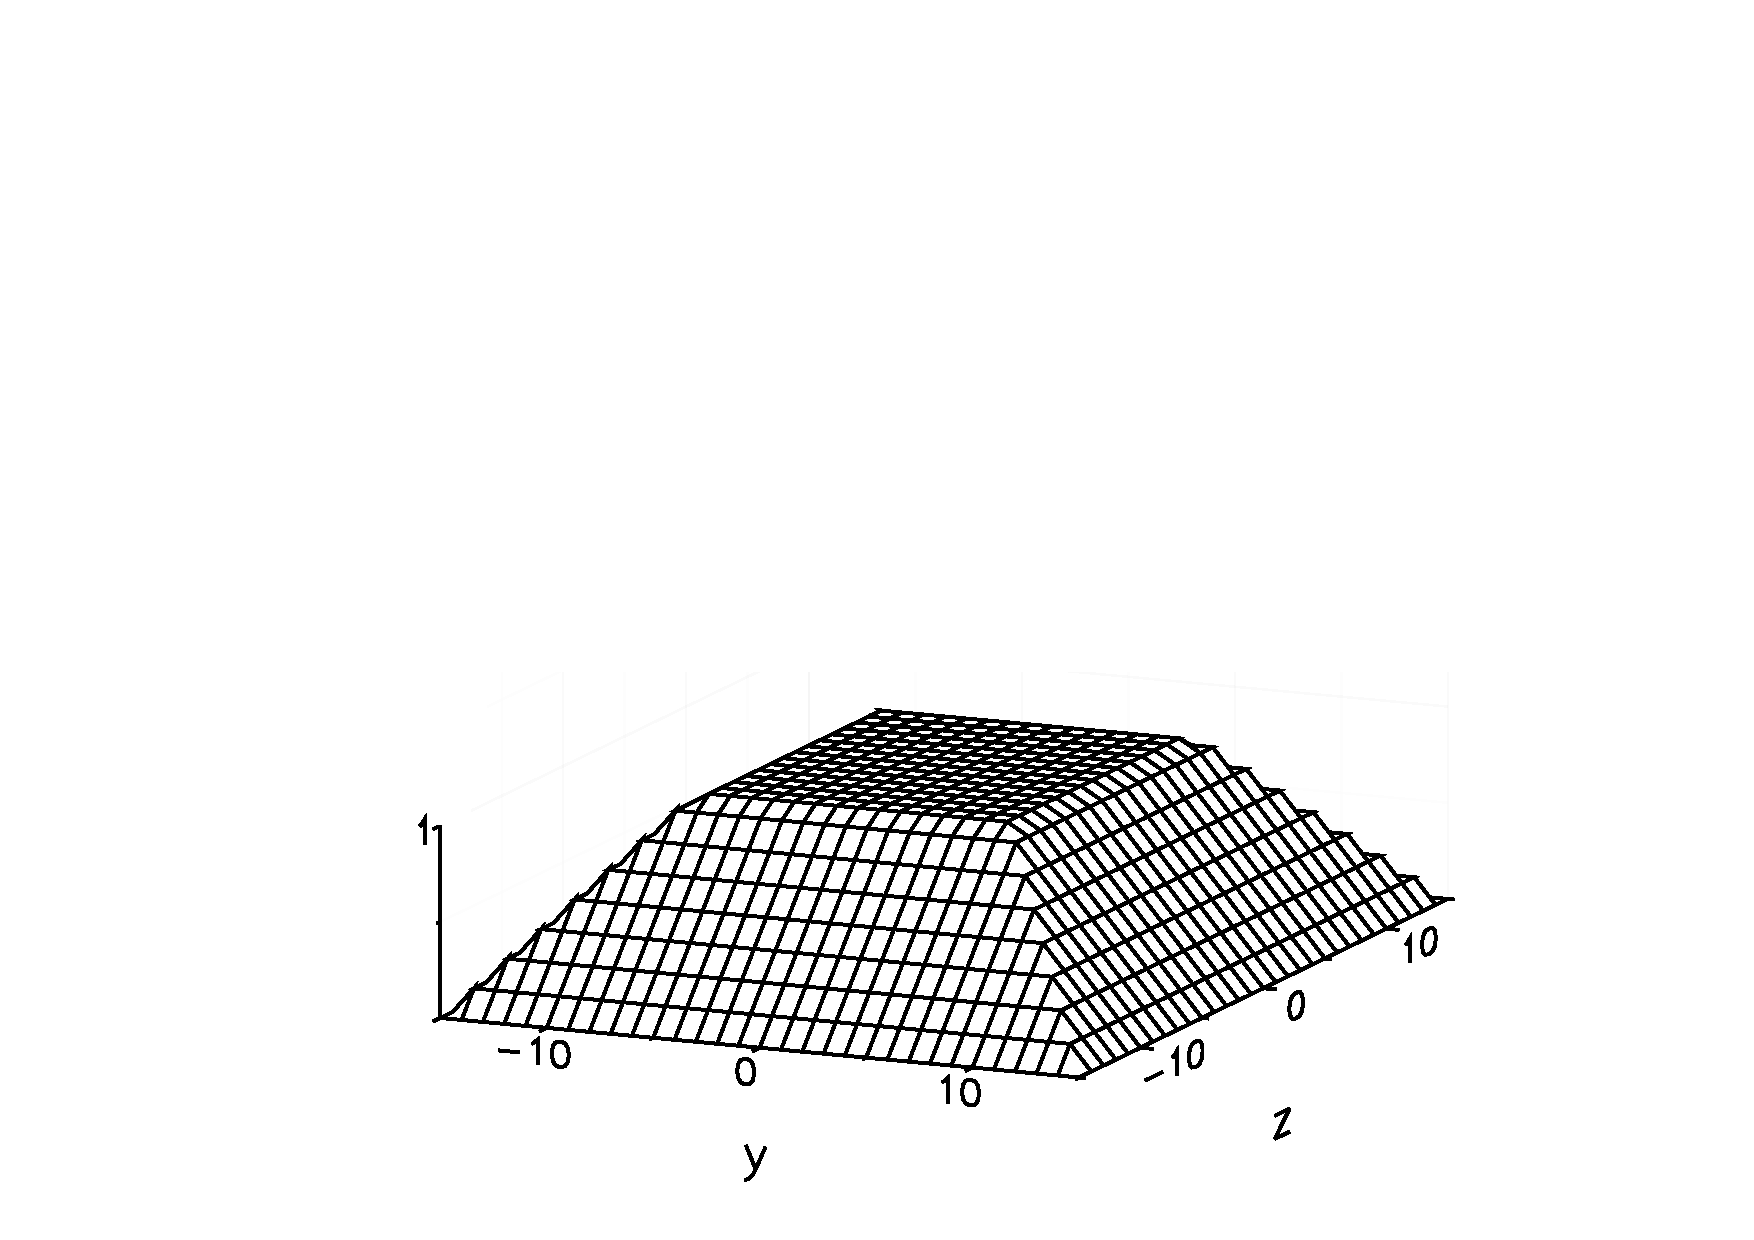
\includegraphics[scale=0.5]{figures/helmholtz/conditions_limites.pdf}
    \caption{Conditions aux limites sur le plan $x = -20$. L'axe vertical
    représente la magnitude de la fonction, non la coordonnée $z$.}
\end{figure}

